\documentclass[11pt]{article}

\usepackage[margin=1in]{geometry}
\usepackage[T1]{fontenc}
\usepackage{lmodern}
\usepackage{microtype}
\usepackage{graphicx}
\usepackage{booktabs}
\usepackage{amsmath}
\usepackage{xcolor}
\usepackage[most]{tcolorbox}
\usepackage{caption}
\usepackage{enumitem}
\usepackage{fancyhdr}
\usepackage[hidelinks]{hyperref}

\newcommand{\Nparticipants}{1,158}
\newcommand{\Nprograms}{30}
\newcommand{\Ntrain}{794}
\newcommand{\Ntest}{364}
\newcommand{\BaseRate}{48\%}
\newcommand{\AUCpre}{0.62}
\newcommand{\AUCfull}{0.69}
\newcommand{\BrierPre}{0.238}
\newcommand{\BrierFull}{0.220}
\newcommand{\ProgCorr}{0.35}
\newcommand{\CovCashflow}{82\%}
\newcommand{\CovPayments}{71\%}
\newcommand{\CovTouchpoints}{66\%}
\newcommand{\ORIntercept}{0.87}
\newcommand{\PIntercept}{= 0.223}
\newcommand{\ORIncomeRegularity}{1.51}
\newcommand{\PIncomeRegularity}{< 0.001}
\newcommand{\ORCashBuffer}{0.96}
\newcommand{\PCashBuffer}{= 0.695}
\newcommand{\ORBalanceVolatility}{0.76}
\newcommand{\PBalanceVolatility}{= 0.006}
\newcommand{\ORRentOnTime}{1.20}
\newcommand{\PRentOnTime}{= 0.072}
\newcommand{\ORUtilityOnTime}{0.99}
\newcommand{\PUtilityOnTime}{= 0.959}
\newcommand{\ORPaymentGapFreq}{0.90}
\newcommand{\PPaymentGapFreq}{= 0.303}
\newcommand{\ORConsentedVisits}{1.37}
\newcommand{\PConsentedVisits}{= 0.011}
\newcommand{\OROptinResponse}{1.45}
\newcommand{\POptinResponse}{= 0.004}
\newcommand{\ORRelationshipDays}{1.27}
\newcommand{\PRelationshipDays}{= 0.060}
\newcommand{\ORMissingCashFlow}{0.89}
\newcommand{\PMissingCashFlow}{= 0.565}
\newcommand{\ORMissingPayments}{0.96}
\newcommand{\PMissingPayments}{= 0.785}
\newcommand{\ORMissingTouchpoints}{1.17}
\newcommand{\PMissingTouchpoints}{= 0.317}
\newcommand{\ORPreIntercept}{0.94}
\newcommand{\PPreIntercept}{= 0.492}
\newcommand{\ORPreIncomeRegularity}{1.57}
\newcommand{\PPreIncomeRegularity}{< 0.001}
\newcommand{\ORPreCashBuffer}{0.98}
\newcommand{\PPreCashBuffer}{= 0.818}
\newcommand{\ORPreBalanceVolatility}{0.79}
\newcommand{\PPreBalanceVolatility}{= 0.015}
\newcommand{\ORPreRentOnTime}{1.22}
\newcommand{\PPreRentOnTime}{= 0.050}
\newcommand{\ORPreUtilityOnTime}{0.99}
\newcommand{\PPreUtilityOnTime}{= 0.922}
\newcommand{\ORPrePaymentGapFreq}{0.86}
\newcommand{\PPrePaymentGapFreq}{= 0.147}
\newcommand{\ORPreMissingCashFlow}{0.90}
\newcommand{\PPreMissingCashFlow}{= 0.560}
\newcommand{\ORPreMissingPayments}{0.95}
\newcommand{\PPreMissingPayments}{= 0.754}


\definecolor{mcred}{HTML}{EB001B}
\definecolor{mcorange}{HTML}{F79E1B}
\definecolor{warnbg}{HTML}{FDF0D8}
\definecolor{warnink}{HTML}{9A5B00}

\captionsetup{font=small, labelfont=bf}
\setlist{nosep, leftmargin=1.4em}

\pagestyle{fancy}
\fancyhf{}
\renewcommand{\headrulewidth}{0pt}
\fancyfoot[L]{\scriptsize\color{warnink}SYNTHETIC DEMONSTRATION: no real participant data or empirical findings}
\fancyfoot[R]{\scriptsize\thepage}

\newtcolorbox{takeaway}{colback=white, colframe=mcred, boxrule=1pt, arc=2pt,
  left=8pt, right=8pt, top=6pt, bottom=6pt}

\title{\vspace{-1.5em}\textbf{Which Signals Predict Whether People Come Back?}\\[0.3em]
\large Modeling 90-day retention in community financial-education programs\\
to decide where outreach should start}
\author{LEAD ASPIRE 2026 Team\thanks{Replace with team member names and affiliations.}}
\date{October 2026}

\begin{document}
\maketitle
\thispagestyle{fancy}

\begin{tcolorbox}[colback=warnbg, colframe=warnink, boxrule=0.6pt, arc=2pt,
  left=6pt, right=6pt, top=3pt, bottom=3pt]
\small\color{warnink}\textbf{Synthetic demonstration.} The data below is simulated to demonstrate
the analysis pipeline. The models, statistics and validation are real computations on that
simulated data. None of the results describe real people, places or programs.
\end{tcolorbox}

\begin{abstract}
\noindent
Bank CRMs start recording at account opening, so the months of workshops and community
contact before that leave no data, and banks have no evidence about where outreach is worth
running. We asked which signals predict whether a participant in a financial-education program
\emph{comes back} within 90 days, our working measure of trust. We fit logistic regressions to
\Nparticipants{} consenting participants from \Nprograms{} past programs (simulated) and tested
them on \Ntest{} held-out participants. Among signals that exist \emph{before} any contact, two
were clearly significant: \textbf{income regularity} (odds ratio \ORPreIncomeRegularity{} per
standard deviation, $p \PPreIncomeRegularity$) and \textbf{balance volatility} (OR
\ORPreBalanceVolatility{}, $p \PPreBalanceVolatility$). Rent paid on time was borderline
(OR \ORPreRentOnTime{}, $p \PPreRentOnTime$). Early relationship touchpoints raised predictive
accuracy (AUC \AUCpre{} $\rightarrow$ \AUCfull{}) but only exist after contact. We therefore use
the pre-contact signals to choose \emph{where} to run outreach, and the touchpoints to decide
\emph{who to follow up with} once people have opted in.
\end{abstract}

\begin{figure}[h]
  \centering
  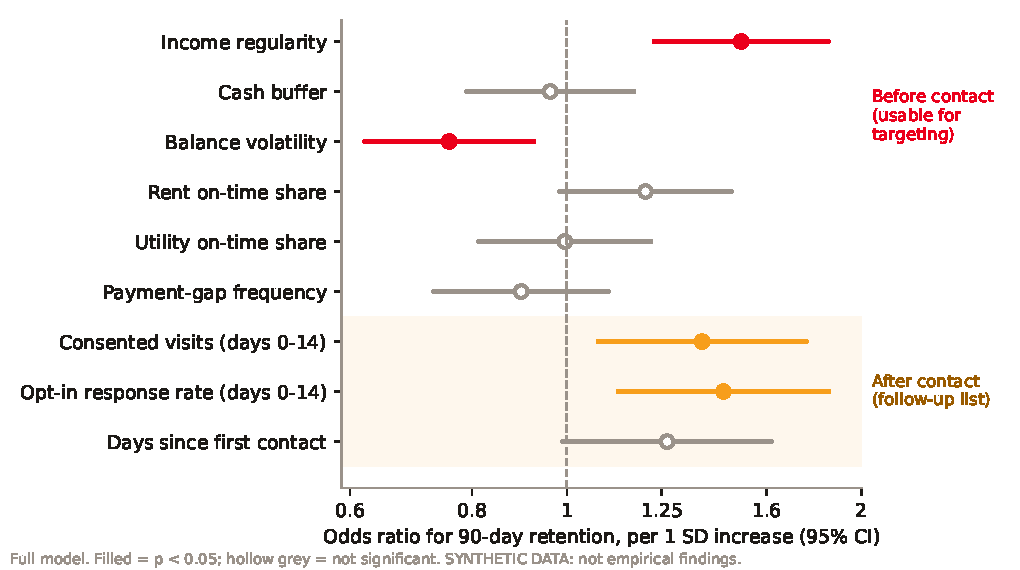
\includegraphics[width=0.92\linewidth]{figures/fig1_odds_ratios.pdf}
  \caption{\textbf{Steady cash flow predicts retention before contact; early engagement predicts it
  after.} Odds ratio for 90-day retention per one-standard-deviation increase in each signal, with
  95\% confidence intervals (full model). Values above 1 mean higher retention. Red: significant
  signals available before contact. Orange: significant signals available only after contact.
  Grey: not significant at $p<0.05$.}
  \label{fig:or}
\end{figure}

\section{Question and hypotheses}

\textbf{Question.} Mastercard and its partner banks want to reach underserved communities, but no
lead list exists for people who have never banked with them. Which measurable signals tell us
where outreach is likely to produce lasting engagement?

\textbf{Outcome: 90-day retention.} A consenting program participant counts as retained if they
have at least one additional recorded interaction with the partner bank within 90 days of their
first program interaction. To keep predictors and outcome separate, only interactions on days
15--90 count toward the outcome; days 0--14 are used as predictors. This measures engagement, not
creditworthiness or account opening.

\begin{enumerate}[label=\textbf{H\arabic*.}]
  \item Signals that describe financial behavior before any contact (cash-flow stability and bill
        payment reliability) are associated with higher 90-day retention.
  \item Early relationship touchpoints add predictive information beyond the pre-contact signals.
\end{enumerate}

\section{Method}

\textbf{Data.} \Nparticipants{} consenting participants across \Nprograms{} community
financial-education programs, all simulated. The overall retention rate is \BaseRate. Each
participant has up to nine signals in three families: \emph{cash flow} (income regularity, cash
buffer, balance volatility), \emph{payments} (rent and utility on-time share, payment-gap
frequency) and \emph{touchpoints} (consented visits and opt-in response rate in days 0--14, days
since first contact). Coverage is incomplete, as it would be in practice: cash-flow signals are
available for \CovCashflow{} of participants, payments for \CovPayments{} and touchpoints for
\CovTouchpoints.

\textbf{Models.} Two logistic regressions estimate the log-odds of retention:
\[
  \log\frac{P(\text{retained})}{1-P(\text{retained})}
  = \beta_0 + \beta_1 x_1 + \beta_2 x_2 + \dots + \beta_k x_k .
\]
The \emph{pre-contact model} uses the six cash-flow and payment signals. The \emph{full model}
adds the three touchpoint signals. Each signal is standardized, so $e^{\beta_j}$ is the change in
the odds of retention for a one-standard-deviation increase. Missing values are set to the mean,
and a flag for each unavailable signal family is included so that missingness cannot bias the
other coefficients. Models are fit by maximum likelihood on a random 70\% of participants
($n=\Ntrain$); significance uses Wald tests.

\textbf{Validation.} On the held-out 30\% ($n=\Ntest$) we measure discrimination (AUC: the
chance a retained participant scores higher than a non-retained one; 0.5 is a coin flip) and
calibration (Brier score and observed versus predicted retention).

\section{Results}

\begin{table}[h]
\centering\small
\caption{Estimated coefficients ($\beta$, log-odds per standard deviation). Significance:
* $p<0.05$, ** $p<0.01$, *** $p<0.001$.}
\label{tab:coefs}
\begin{tabular}{lrrrrrr}
\toprule
 & \multicolumn{3}{c}{Pre-contact model} & \multicolumn{3}{c}{Full model} \\
\cmidrule(lr){2-4}\cmidrule(lr){5-7}
Signal & $\beta$ & SE & $p$ & $\beta$ & SE & $p$ \\
\midrule
Intercept & $-$0.07 & 0.10 & 0.492 & $-$0.14 & 0.12 & 0.223 \\
Income regularity & $+$0.45*** & 0.10 & $<$0.001 & $+$0.41*** & 0.10 & $<$0.001 \\
Cash buffer & $-$0.02 & 0.10 & 0.818 & $-$0.04 & 0.10 & 0.695 \\
Balance volatility & $-$0.24* & 0.10 & 0.015 & $-$0.28** & 0.10 & 0.006 \\
Rent on-time share & $+$0.20* & 0.10 & 0.050 & $+$0.18 & 0.10 & 0.072 \\
Utility on-time share & $-$0.01 & 0.10 & 0.922 & $-$0.01 & 0.10 & 0.959 \\
Payment-gap frequency & $-$0.15 & 0.10 & 0.147 & $-$0.11 & 0.10 & 0.303 \\
Consented visits (days 0--14) & \multicolumn{3}{c}{---} & $+$0.32* & 0.12 & 0.011 \\
Opt-in response rate (days 0--14) & \multicolumn{3}{c}{---} & $+$0.37** & 0.13 & 0.004 \\
Days since first contact & \multicolumn{3}{c}{---} & $+$0.24 & 0.13 & 0.060 \\
Cash flow unavailable & $-$0.11 & 0.19 & 0.560 & $-$0.11 & 0.19 & 0.565 \\
Payments unavailable & $-$0.05 & 0.16 & 0.754 & $-$0.05 & 0.17 & 0.785 \\
Touchpoints unavailable & \multicolumn{3}{c}{---} & $+$0.16 & 0.16 & 0.317 \\
\midrule
Held-out AUC & \multicolumn{3}{c}{0.62} & \multicolumn{3}{c}{0.69} \\
Held-out Brier score & \multicolumn{3}{c}{0.238} & \multicolumn{3}{c}{0.220} \\
\bottomrule
\end{tabular}

\end{table}

\textbf{H1 is supported for cash-flow stability.} Participants with steadier income were more
likely to return (OR \ORPreIncomeRegularity), and those with more volatile balances less likely
(OR \ORPreBalanceVolatility). Rent on-time share was borderline in the pre-contact model
($p \PPreRentOnTime$) and not significant in the full model ($p \PRentOnTime$). Cash buffer,
utility payments and payment gaps showed no detectable association.

\textbf{H2 is supported.} Consented visits (OR \ORConsentedVisits) and opt-in response rate
(OR \OROptinResponse) in the first two weeks were significant, and adding touchpoints raised the
held-out AUC from \AUCpre{} to \AUCfull. Both models are well calibrated
(Figure~\ref{fig:val}): when they predict 50\% retention, close to 50\% of participants return.

\begin{figure}[h]
  \centering
  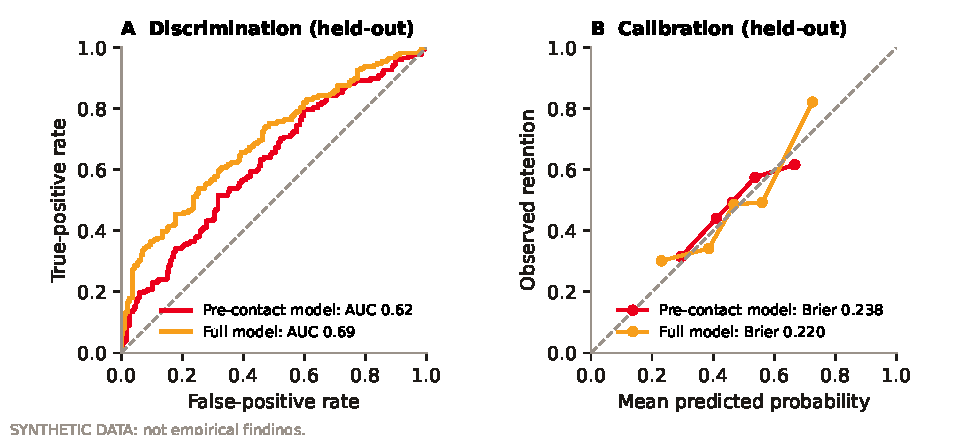
\includegraphics[width=0.85\linewidth]{figures/fig2_validation.pdf}
  \caption{\textbf{Both models beat chance on participants they never saw, and their
  probabilities can be trusted.} (A) ROC curves on held-out participants. (B) Observed retention
  against predicted probability, in five equal-size groups; the dashed line is perfect
  calibration.}
  \label{fig:val}
\end{figure}

\textbf{From people to places.} Averaging each program's pre-contact model score across its
participants tracks the program's retention rate (Figure~\ref{fig:prog}; $r = \ProgCorr$ across
programs with at least 15 participants). This is the link the product relies on: area-level
aggregates of the same cash-flow signals can rank places before anyone is contacted.

\begin{figure}[h]
  \centering
  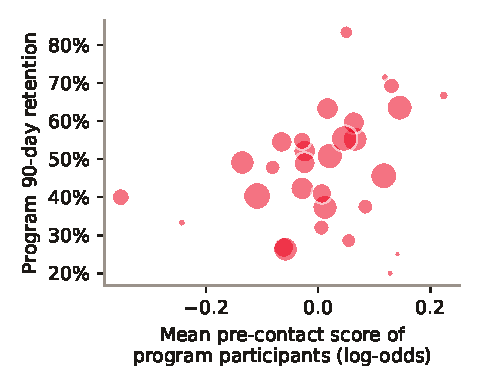
\includegraphics[width=0.42\linewidth]{figures/fig3_programs.pdf}
  \caption{\textbf{Programs whose participants had steadier finances retained more people.}
  Each point is one program; point size reflects the number of participants.}
  \label{fig:prog}
\end{figure}

\section{Limitations}
\begin{itemize}
  \item All data is simulated. The pipeline is ready; the real coefficients will come from the
        pilot.
  \item Associations are not causes. Steady income may mark people with more time to attend,
        not people who trust the bank more.
  \item Effects are modest (AUC \AUCpre{} before contact). The model points to promising places
        to test outreach; it does not predict any individual's behavior.
  \item Figure~\ref{fig:prog} is in-sample. Applying participant-level effects to area averages
        assumes the relationship holds at area level, which must be checked with new programs.
\end{itemize}

\section{Conclusion}

\begin{takeaway}
\textbf{Two signals that exist before any contact, steady income and stable balances, are the
most informative predictors of whether people come back.} We use them, with their estimated
weights, to rank communities for the next outreach pilot. Early engagement is an even stronger
predictor but only exists after contact, so it powers the retention follow-up list instead.
Every pilot adds real outcomes that replace these simulated estimates.
\end{takeaway}

\noindent
\textbf{How the product uses this.}
\begin{enumerate}
  \item \textbf{Where to go:} score candidate areas with the pre-contact coefficients applied to
        area-level aggregates of income regularity, balance volatility and rent on-time share.
  \item \textbf{Who to follow up with:} after people opt in, use the full model to flag
        participants with low early engagement before day 45.
  \item \textbf{Learn:} add each pilot's measured 90-day retention to the dataset and re-fit.
\end{enumerate}

\end{document}
